\documentclass[10pt,letterpaper]{article}

% Scholarly typography: NewTX text and mathematics throughout.
\usepackage[T1]{fontenc}
\usepackage{amsmath,amssymb,amsthm,mathtools}
\usepackage{newtxtext}
\usepackage{newtxmath}
\usepackage{bm}
\usepackage[letterpaper,top=0.78in,bottom=0.80in,left=0.72in,right=0.72in,headheight=13pt,headsep=0.20in,footskip=0.37in]{geometry}
\setlength{\columnsep}{0.28in}
\setlength{\columnseprule}{0pt}
\usepackage{microtype}
\usepackage{xcolor}
\definecolor{VelvetBlue}{HTML}{000D3C}
\definecolor{MutedInk}{HTML}{525864}
\definecolor{TrendOrange}{HTML}{B75A3C}
\definecolor{MeanGreen}{HTML}{257A62}
\usepackage{booktabs,needspace}
\usepackage{dblfloatfix}
\usepackage{enumitem}
\usepackage{titlesec}
\usepackage{fancyhdr}
\usepackage{caption}
\usepackage{pgfplots}
\pgfplotsset{compat=1.18}
\usepackage[colorlinks=true,linkcolor=VelvetBlue,urlcolor=VelvetBlue,citecolor=VelvetBlue]{hyperref}
\hypersetup{pdftitle={Smoothness-Integrated Trend Distances with Nonzero Difference Drift},pdfsubject={PLS smoothing, functional distances, nonzero difference drift}}

% Hierarchy and restrained accents; avoid decorative frames around equations.
\titleformat{\section}[hang]
  {\color{VelvetBlue}\normalsize\bfseries}
  {\thesection}{0.75em}{}
  [\vspace{.26ex}{\color{VelvetBlue!23}\titlerule[0.35pt]}]
\titlespacing*{\section}{0pt}{2.6ex plus .7ex minus .2ex}{1.0ex}
\titleformat{\subsection}[hang]
  {\color{VelvetBlue}\normalsize\bfseries}
  {\thesubsection}{0.7em}{}
\titlespacing*{\subsection}{0pt}{2.0ex plus .4ex minus .2ex}{0.7ex}
\titleformat{\paragraph}[runin]
  {\normalfont\bfseries\color{VelvetBlue}}
  {}{0pt}{}
\titlespacing*{\paragraph}{0pt}{1.6ex plus .4ex minus .2ex}{0.65em}

\fancyhf{}
\fancyhead[L]{\scriptsize\textcolor{MutedInk}{SMOOTHNESS-INTEGRATED TREND DISTANCES}}
\fancyhead[R]{\scriptsize\textcolor{VelvetBlue}{RESEARCH NOTE}}
\fancyfoot[C]{\footnotesize\textcolor{MutedInk}{\thepage}}
\renewcommand{\headrulewidth}{0.35pt}
\renewcommand{\footrulewidth}{0pt}
\pagestyle{fancy}
\fancypagestyle{firstpage}{\fancyhf{}\fancyfoot[C]{\footnotesize\textcolor{MutedInk}{\thepage}}\renewcommand{\headrulewidth}{0pt}}

\captionsetup{font=footnotesize,labelfont={bf,color=VelvetBlue},labelsep=period,skip=5pt}
\setlength{\parindent}{1.05em}
\setlength{\parskip}{0pt plus .3pt}
\setlength{\abovedisplayskip}{7pt plus 2pt minus 2pt}
\setlength{\belowdisplayskip}{7pt plus 2pt minus 2pt}
\setlength{\abovedisplayshortskip}{4pt plus 2pt minus 1pt}
\setlength{\belowdisplayshortskip}{5pt plus 2pt minus 2pt}
\setlist[enumerate]{topsep=5pt,itemsep=3pt,parsep=0pt,leftmargin=2.0em}
\renewcommand{\arraystretch}{1.14}

\newcommand{\R}{\mathbb{R}}
\newcommand{\Hilbert}{\mathcal{H}}
\newcommand{\norm}[1]{\left\lVert#1\right\rVert}
\newcommand{\ip}[2]{\left\langle#1,#2\right\rangle}
\DeclareMathOperator{\diag}{diag}

\begin{document}
\twocolumn[{\begin{@twocolumnfalse}
\thispagestyle{firstpage}
\noindent{\sffamily\color{VelvetBlue}\bfseries\scriptsize RESEARCH NOTE \enspace/\enspace WORKING DRAFT}
\par\vspace{0.75em}
\noindent{\fontsize{19}{23}\selectfont\bfseries\color{VelvetBlue}
Smoothness-Integrated Trend Distances\\[2pt]
with Nonzero Difference Drift\par}
\vspace{0.9em}
\noindent{\color{MutedInk}\itshape Mathematical formulation and numerical implications\par}
\vspace{1.0em}
\noindent{\color{VelvetBlue!30}\rule{\linewidth}{0.6pt}}
\vspace{0.5em}

\begingroup
\small
\noindent{\color{VelvetBlue}\bfseries Abstract}\par\vspace{0.4em}
\noindent
We compare time series using entire smoothness-indexed families of
penalized least-squares (PLS) trends. Crucially, the penalized $d$th
finite differences need not be centered at zero: we allow a nonzero
reference drift $\mu$ in the objective
$\|y-\tau\|_2^2+\lambda\|D_d\tau-\mu\bm{1}\|_2^2$.
This leads to an affine trend estimator, a nonzero-drift smoothness limit,
and a necessary distinction between the \emph{penalty drift} $\mu$ and
the \emph{signed mean difference of two fitted trends} $\mu_\Delta$.
Using the normalized coordinate $S\in[0,1]$ of the companion numerical
study, we construct Hilbert-space global distances, time-local rolling
distances, and smoothness--time dissimilarity surfaces. We give exact
spectral representations with matching drift and a corrected formula
for unequal drifts, plus a numerical example and monitoring cautions.
\par
\endgroup
\vspace{1.2em}
\end{@twocolumnfalse}}]

\section{Penalized trend estimation with nonzero difference drift}
\label{sec:pls}
\textbf{Notation.} Let $y=(y_1,\ldots,y_N)^\top\in\R^N$ be an observed
series at $N$ aligned times; let $d$ be a difference order with
$1\le d<N$; let $D_d\in\R^{(N-d)\times N}$ represent the $d$th
forward finite-difference operator; and let
\begin{equation}\label{eq:roughness}
 Q=D_d^\top D_d\in\R^{N\times N},\qquad
 \bm{1}_r=(1,\ldots,1)^\top\in\R^r.
\end{equation}
The matrix $Q$ is symmetric positive semidefinite and $D_d$ has full
row rank. Following the general nonzero-reference-difference formulation
of Guerrero, introduce $\mu\in\R$, the target mean or reference level of
the \emph{$d$th differences}. Thus the penalty target is
$\mu\bm{1}_{N-d}$, not a scalar subtracted from a vector. For
$\lambda\ge0$, define
\begin{equation}\label{eq:pls}
\widehat{\bm\tau}_{\lambda,\mu}(y)
=\underset{u\in\R^N}{\operatorname{argmin}}
\left\{\|y-u\|_2^2+
\lambda\|D_du-\mu\bm{1}_{N-d}\|_2^2\right\}.
\end{equation}
The normal equations are
\begin{equation}\label{eq:normal}
 (I_N+\lambda Q)\widehat{\bm\tau}_{\lambda,\mu}
 =y+\lambda\mu D_d^\top\bm{1}_{N-d}.
\end{equation}
Therefore, with the numerical manuscript's smoothing-matrix notation,
\begin{equation}\label{eq:H}
 H_\lambda=(I_N+\lambda Q)^{-1},\qquad
 \widehat{\bm\tau}_{\lambda,\mu}(y)
 =H_\lambda\bigl(y+\lambda\mu D_d^\top\bm{1}_{N-d}\bigr).
\end{equation}
The solution is unique because $I_N+\lambda Q$ is positive definite.
At $\mu=0$ we recover the usual formula $H_\lambda y$ from the
companion numerical paper; setting $\mu=0$ is an \emph{assumption},
not a general identity.

\paragraph{The drift changes the limiting trend.}
Define the minimum-norm vector satisfying the reference-difference
constraint,
\begin{equation}\label{eq:bmu}
\begin{aligned}
 b_\mu&=\mu D_d^\top(D_dD_d^\top)^{-1}\bm{1}_{N-d},\\
 D_db_\mu&=\mu\bm{1}_{N-d},\quad b_\mu\perp\ker(D_d).
\end{aligned}
\end{equation}
Since $Qb_\mu=\mu D_d^\top\bm{1}_{N-d}$, equation~\eqref{eq:H}
can be rearranged as
\begin{equation}\label{eq:affine}
\widehat{\bm\tau}_{\lambda,\mu}(y)
 =b_\mu+H_\lambda(y-b_\mu).
\end{equation}
Consequently,
\begin{equation}\label{eq:limits}
\widehat{\bm\tau}_{0,\mu}(y)=y,\qquad
\lim_{\lambda\to\infty}\widehat{\bm\tau}_{\lambda,\mu}(y)
=P_{\ker(D_d)}y+b_\mu.
\end{equation}
For $d=1$, a nonzero $\mu$ allows a linear limiting trend; for
$d=2$, it allows a quadratic limiting trend. Thus, unlike the case
$\mu=0$, strong smoothing need not make the $d$th difference vanish.

\paragraph{Known versus estimated drift.}
The drift $\mu$ may be specified in advance, shared across series,
or estimated separately. A simple estimate from the observed
$d$th differences, as in Guerrero, is
\begin{equation}\label{eq:muhat}
 \widehat\mu(y)=\frac{1}{N-d}\bm{1}_{N-d}^\top D_dy.
\end{equation}
If $\mu$ is estimated from $y$, the overall map from $y$ to the trend
is still linear for this choice, but its matrix is not generally
$H_\lambda$; specifically,
\begin{equation}\label{eq:effective_H}
 \widehat{\bm\tau}_{\lambda,\widehat\mu(y)}(y)
 =\underbrace{H_\lambda\!\left[I_N+
 \frac{\lambda}{N-d}D_d^\top\bm{1}_{N-d}
 \bm{1}_{N-d}^\top D_d\right]}_{\widetilde H_\lambda}y.
\end{equation}
The distinction affects spectral formulas and the interpretation of
trace-based effective degrees of freedom.

\section{The normalized smoothness coordinate \texorpdfstring{$S$}{S}}
\label{sec:smoothness}
We use the smoothness coordinate $S$ from the companion manuscript.
Because $D_d$ has rank $N-d$, the matrix $Q$ has $d$ zero eigenvalues
and $N-d$ positive eigenvalues $\rho_j>0$. Define
\begin{equation}\label{eq:S}
 S(\lambda;N,d)
 =\frac{N}{N-d}\left(1-\frac{\operatorname{tr}(H_\lambda)}{N}\right)
 =1-\frac{1}{N-d}\sum_{j=1}^{N-d}
      \frac{1}{1+\lambda\rho_j}.
\end{equation}
Then $S(0)=0$, $S(\infty)=1$, and $S'(\lambda)>0$ for finite
$\lambda\ge0$. Thus its inverse $\lambda(S)$ exists for $0\le S<1$;
$\lambda(1):=\infty$ is interpreted by a limit. Holding $N$, $d$,
and $D_d$ fixed gives a \emph{common, data-independent calibration}
across both series. For a supplied drift $\mu$ define the full trend
path
\begin{equation}\label{eq:path}
 \bm\tau_y(S;\mu)
 :=\widehat{\bm\tau}_{\lambda(S),\mu}(y),
 \qquad S\in[0,1].
\end{equation}
When a distinct drift $\mu_i$ is used for each series, write
$\bm\tau_{y_i}(S):=\bm\tau_{y_i}(S;\mu_i)$.
The trace coordinate in \eqref{eq:S} is defined using $H_\lambda$;
for an estimated, data-dependent drift the effective linear map is
$\widetilde H_\lambda$ in \eqref{eq:effective_H}, so the trace of
$H_\lambda$ should be interpreted as the chosen \emph{nominal
Guerrero smoothness coordinate}, not automatically as the effective
degrees of freedom of that adjusted estimator.

\section{A global distance between entire trend families}
\label{sec:global}
The trend path is a vector-valued function of the smoothness
coordinate. Work in the Hilbert space
\begin{equation}
 \Hilbert=L^2([0,1];\R^N),\qquad
 \ip{f}{g}_{\Hilbert}=\frac1N\int_0^1f(S)^\top g(S)\,dS.
\end{equation}
Since $\|H_\lambda\|_{2\to2}\le1$ and $b_\mu$ is fixed,
\eqref{eq:affine} shows that each trend path is bounded and therefore
belongs to $\Hilbert$. Given series $y_1,y_2\in\R^N$, define
\begin{equation}\label{eq:main}
\mathcal D_{\mathrm{PLS}}(y_1,y_2)
 =\left[\frac1N\int_0^1
 \|\bm\tau_{y_1}(S)-\bm\tau_{y_2}(S)\|_2^2\,dS
 \right]^{1/2}.
\end{equation}
This measures disagreement over \emph{all} smoothing levels.
The pointwise-in-smoothness RMS distance is
\begin{equation}\label{eq:pointwise}
 d(S)=\frac1{\sqrt N}\|\bm\tau_{y_1}(S)-\bm\tau_{y_2}(S)\|_2,
 \qquad \mathcal D_{\mathrm{PLS}}^2=\int_0^1d(S)^2\,dS.
\end{equation}
The Hilbert-space norm is a metric on trend paths (modulo equality
almost everywhere). Its pullback to observed series is a pseudometric,
and is a metric whenever the chosen smoothing-and-drift mapping is
injective almost everywhere. In particular, if the same fixed $\mu$
and the same calibration are used, the result is a metric on $\R^N$.

\section{A nonzero \emph{mean difference} between fitted trends}
\label{sec:mean}
Here the symbol $\mu_\Delta$ is intentionally \emph{different} from
the penalty-drift parameter $\mu$ in Section~\ref{sec:pls}.
Let $\bm 1_N$ be the constant vector and set
\begin{equation}\label{eq:mean_delta}
\bm\Delta(S)=\bm\tau_{y_2}(S)-\bm\tau_{y_1}(S),\qquad
\mu_\Delta(S)=\frac1N\bm{1}_N^\top\bm\Delta(S).
\end{equation}
No zero-mean assumption is made. Split into an average level
and centered discrepancy,
\begin{equation}\label{eq:centered_delta}
 \bm\Delta(S)=\mu_\Delta(S)\bm{1}_N+
 \widetilde{\bm\Delta}(S),\qquad
 \bm{1}_N^\top\widetilde{\bm\Delta}(S)=0.
\end{equation}
Orthogonality gives the global decomposition
\begin{equation}\label{eq:mean_shape_global}
\mathcal D_{\mathrm{PLS}}^2
 =\underbrace{\int_0^1\mu_\Delta(S)^2\,dS}_{\mathcal D_{\mathrm{level}}^2}
 +\underbrace{\frac1N\int_0^1\|\widetilde{\bm\Delta}(S)\|_2^2\,dS}_{\mathcal D_{\mathrm{shape}}^2}.
\end{equation}
The scale-averaged \emph{signed} level gap is
\begin{equation}\label{eq:signed_global_mean}
\overline\mu_\Delta=\int_0^1\mu_\Delta(S)\,dS.
\end{equation}
This signed summary preserves direction; the nonnegative level
component $\mathcal D_{\mathrm{level}}$ does not.

\paragraph{Why nonzero penalty drift does not destroy mean preservation.}
For every difference order $d\ge1$, $D_d\bm{1}_N=0$. Hence
$H_\lambda\bm{1}_N=\bm{1}_N$ and
$\bm{1}_N^\top H_\lambda D_d^\top=0$, regardless of $\mu$.
Thus the affine estimator in \eqref{eq:H} satisfies
\begin{equation}\label{eq:mean_preservation}
 \frac1N\bm{1}_N^\top\bm\tau_y(S;\mu)=\overline y
 \qquad\text{for all }S\in[0,1]\text{ and all }\mu.
\end{equation}
Consequently, even for \emph{different, nonzero} drifts $\mu_1$
and $\mu_2$,
\begin{equation}\label{eq:constant_mean_gap}
 \mu_\Delta(S)=\overline y_2-\overline y_1=:\mu_0,
 \qquad \mathcal D_{\mathrm{PLS}}^2=\mu_0^2+\mathcal D_{\mathrm{shape}}^2.
\end{equation}
Here $\mu_0$ is an observed-level mean difference; it is \emph{not}
the penalty drift $\mu$. These identities require the ordinary
unweighted least-squares data term and a difference operator
annihilating constants.

\section{Numerical integration in the normalized coordinate}
\label{sec:numerical}
For a grid $0=S_0<S_1<\cdots<S_M=1$, calculate both trend paths,
including their chosen reference drifts, and apply trapezoidal
quadrature:
\begin{equation}\label{eq:quad}
 \mathcal D_{\mathrm{PLS}}(y_1,y_2)
 \approx\left\{\sum_{j=0}^{M-1}\frac{S_{j+1}-S_j}{2}
 [d(S_j)^2+d(S_{j+1})^2]\right\}^{1/2}.
\end{equation}
A first grid is $S_j=j/10$; refine and check numerical stability.
The endpoint $S=1$ must be evaluated from \eqref{eq:limits}, not by
blindly replacing $\lambda=\infty$ with a large finite number.

\section{Spectral form: common and unequal drifts}
\label{sec:spectral}
Assume the same $N,d,D_d$ and hence the same $\lambda(S)$ for both
series. Let $\Delta y=y_2-y_1$, let
$b_i=b_{\mu_i}$ from \eqref{eq:bmu}, and let $\Delta b=b_2-b_1$.
Equation~\eqref{eq:affine} gives
\begin{equation}\label{eq:spectral_difference}
 \bm\Delta(S)
 =H_{\lambda(S)}(\Delta y-\Delta b)+\Delta b.
\end{equation}
Write $Q=U\diag(\rho_1,\ldots,\rho_N)U^\top$, with $U^\top U=I$,
and let $u_j$ denote column $j$ of $U$. The general formula is
\begin{equation}\label{eq:spectral_affine}
\begin{aligned}
\mathcal D_{\mathrm{PLS}}^2
 &=\frac1N\sum_{j=1}^N\int_0^1\Biggl[
 \frac{u_j^\top\Delta y}{1+\lambda(S)\rho_j}\\
 &\quad+\left(1-\frac1{1+\lambda(S)\rho_j}\right)
 u_j^\top\Delta b\Biggr]^2\,dS.
\end{aligned}
\end{equation}
In particular, if the two reference drifts are equal
($\mu_1=\mu_2$, not necessarily zero), then $\Delta b=0$ and
\begin{equation}\label{eq:M}
 \mathcal D_{\mathrm{PLS}}^2=\frac1N\Delta y^\top M\Delta y,
 \qquad M=\int_0^1H_{\lambda(S)}^2\,dS,
\end{equation}
with the simpler spectral weights
\begin{equation}\label{eq:spectral}
 \mathcal D_{\mathrm{PLS}}^2
 =\frac1N\sum_{j=1}^N\left[\int_0^1
 \frac{dS}{(1+\lambda(S)\rho_j)^2}\right]
 (u_j^\top\Delta y)^2.
\end{equation}
A nonzero \emph{common} $\mu$ cancels from the difference and leaves
this spectral metric unchanged. If $\mu_i$ are estimated separately
from the data, $\Delta b$ generally does not vanish; use
\eqref{eq:spectral_affine}, not \eqref{eq:spectral}. The nominal
coordinate $S$ is still common when $N,d,D_d$ are fixed. If one
instead calibrates smoothness separately in a data-dependent way, the
single-matrix formulas require further modification.

\section{From global similarity to time-localized differences}
\label{sec:rolling}
Let $t\in\{1,\ldots,N\}$ index aligned observation times and set
\begin{equation}\label{eq:components}
\begin{aligned}
\tau_i(S,t)&=[\bm\tau_{y_i}(S)]_t,\\
\Delta(S,t)&=\tau_2(S,t)-\tau_1(S,t),\\
\delta(S,t)&=|\Delta(S,t)|.
\end{aligned}
\end{equation}
The signed difference $\Delta$ indicates \emph{which} series has a
higher estimated trend, whereas $\delta$ measures the magnitude of the
difference at one time and one smoothing level. Neither quantity alone
is a rolling-window distance.

\subsection{A worked example at one smoothing level}
To illustrate the distinction, fix a smoothness level $S$ and suppose
two seven-point trend vectors are
\begin{equation}\label{eq:example}
\begin{aligned}
\bm\tau_{y_1}(S)&=(1,1,1,1,1,1,1)^\top,\\
\bm\tau_{y_2}(S)&=(1,1,1,1,3,5,7)^\top.
\end{aligned}
\end{equation}
These are \emph{illustrative vectors}, not claimed to be outputs of a
particular PLS estimator. Their absolute difference is
\begin{equation}
  \bigl(\delta(S,1),\ldots,\delta(S,7)\bigr)
  =(0,0,0,0,2,4,6).
\end{equation}
The series coincide for times $1$--$4$ and start differing at time $5$.

\subsection{Scale-specific rolling distance}
Choose a window length $w\in\{1,\ldots,N\}$. For $t=w,\ldots,N$,
define
\begin{equation}\label{eq:scale_time}
  D_w(S,t)
  =\left[\frac1w\sum_{k=t-w+1}^{t}\Delta(S,k)^2\right]^{1/2}.
\end{equation}
The map $(S,t)\mapsto D_w(S,t)$ is a \emph{scale--time dissimilarity
surface}: for each smoothness level it measures the root-mean-square
difference over the most recent $w$ observations. A heatmap of this
surface can distinguish differences that are visible only at some
smoothness levels from those that persist over a broad range of scales.

\Needspace{15\baselineskip}
For the vectors in \eqref{eq:example}, $w=3$ gives
(the signed mean $\mu_3(S,t)$ is defined in
Section~\ref{sec:rolling_mean})
\begin{table*}[t]
\centering\small
\begin{tabular{@{}cccc@{}}
\toprule
Time $t$ & Pointwise $\delta(S,t)$ & Signed $\mu_3(S,t)$ & Rolling $D_3(S,t)$ \\
\midrule
$3$ & $0$ & $0$ & $0$ \\
$4$ & $0$ & $0$ & $0$ \\
$5$ & $2$ & $2/3$ & $\sqrt{4/3}\approx1.155$ \\
$6$ & $4$ & $2$ & $\sqrt{20/3}\approx2.582$ \\
$7$ & $6$ & $4$ & $\sqrt{56/3}\approx4.320$ \\
\bottomrule
\end{tabular}
\caption{Pointwise discrepancy, signed rolling mean, and three-point rolling RMS for the synthetic example.}
\label{tab:rolling}
\end{table*}
The pointwise difference responds immediately at time $5$, while the
rolling RMS accumulates the discrepancy over the selected window.

\begin{figure*}[t]
  \centering
  \begin{minipage}{0.49\linewidth}
  \centering
  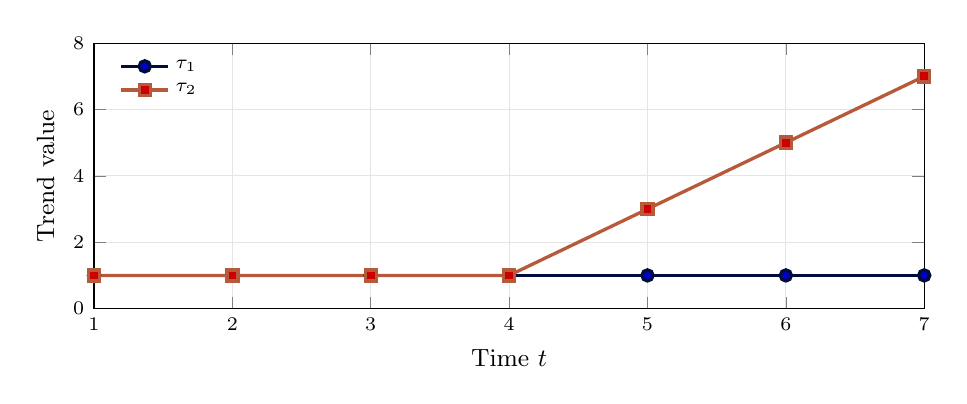
\begin{tikzpicture}
    \begin{axis}[
      width=\linewidth,height=1.95in,
      xlabel={Time $t$},ylabel={Trend value},
      xmin=1,xmax=7,ymin=0,ymax=8,
      xtick={1,...,7},grid=major,
      grid style={gray!20},tick label style={font=\scriptsize},
      label style={font=\small},
      legend style={font=\scriptsize,at={(0.02,0.98)},anchor=north west,
      fill=white,draw=none}]
      \addplot+[mark=*,very thick,color=VelvetBlue]
        coordinates {(1,1)(2,1)(3,1)(4,1)(5,1)(6,1)(7,1)};
      \addlegendentry{$\tau_1$}
      \addplot+[mark=square*,very thick,color=TrendOrange]
        coordinates {(1,1)(2,1)(3,1)(4,1)(5,3)(6,5)(7,7)};
      \addlegendentry{$\tau_2$}
    \end{axis}
  \end{tikzpicture}
  \end{minipage}\hfill
  \begin{minipage}{0.49\linewidth}
  \centering
  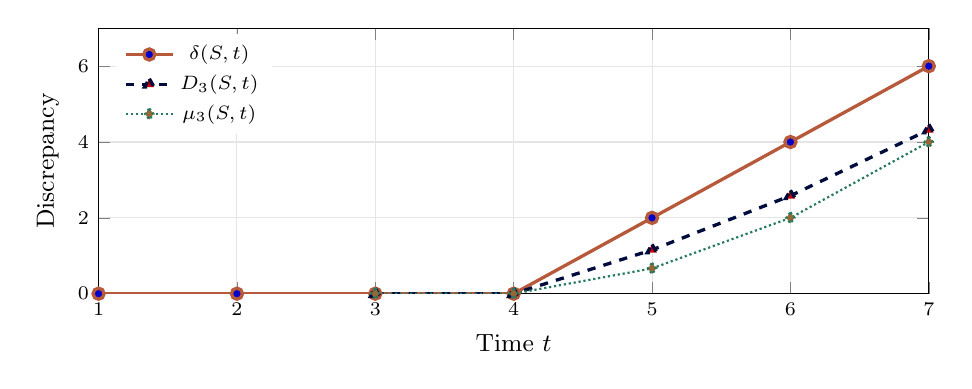
\begin{tikzpicture}
    \begin{axis}[
      width=\linewidth,height=1.95in,
      xlabel={Time $t$},ylabel={Discrepancy},
      xmin=1,xmax=7,ymin=0,ymax=7,
      xtick={1,...,7},grid=major,
      grid style={gray!20},tick label style={font=\scriptsize},
      label style={font=\small},
      legend style={font=\scriptsize,at={(0.02,0.98)},anchor=north west,
      fill=white,draw=none}]
      \addplot+[mark=*,very thick,color=TrendOrange]
        coordinates {(1,0)(2,0)(3,0)(4,0)(5,2)(6,4)(7,6)};
      \addlegendentry{$\delta(S,t)$}
      \addplot+[mark=triangle*,very thick,dashed,color=VelvetBlue]
        coordinates {(3,0)(4,0)(5,1.1547)(6,2.582)(7,4.3205)};
      \addlegendentry{$D_3(S,t)$}
      \addplot+[mark=diamond*,thick,densely dotted,color=MeanGreen]
        coordinates {(3,0)(4,0)(5,0.6667)(6,2)(7,4)};
      \addlegendentry{$\mu_3(S,t)$}
    \end{axis}
  \end{tikzpicture}
  \end{minipage}
  \caption{Synthetic illustration at a fixed smoothness level. Left:
    two trend vectors. Right: the pointwise absolute difference and the
    three-observation rolling RMS and signed rolling mean.}
  \label{fig:rolling-example}
\end{figure*}

\subsection{Rolling signed mean and mean-adjusted variation}
\label{sec:rolling_mean}
To distinguish a persistent directional shift from fluctuating
mismatches, retain the \emph{signed} window mean
\begin{equation}\label{eq:rolling_mean}
  \mu_w(S,t)=\frac1w\sum_{k=t-w+1}^{t}\Delta(S,k).
\end{equation}
Its sign tells us which trend tends to be higher in that window
(recall $\Delta=\tau_2-\tau_1$). Define the within-window centered
mean-square difference using divisor $w$,
\begin{equation}\label{eq:rolling_variation}
  v_w(S,t)=\frac1w\sum_{k=t-w+1}^{t}
              \bigl[\Delta(S,k)-\mu_w(S,t)\bigr]^2.
\end{equation}
Expanding the square and using the definition of $\mu_w$ proves
\begin{equation}\label{eq:rolling_decomp}
  D_w(S,t)^2=\mu_w(S,t)^2+v_w(S,t).
\end{equation}
This decomposition explains \emph{why} the rolling RMS can be large:
either the signed difference has a substantial nonzero mean, or the
differences fluctuate around their mean (or both). It holds even
when the mean is not zero.

\subsection{Rolling distance integrated across all smoothness levels}
Rather than selecting a single $S$, integrate the squared rolling
discrepancy over $S\in[0,1]$:
\begin{equation}\label{eq:rolling_integrated}
\begin{aligned}
\mathcal D_w(t)^2
 &=\int_0^1 D_w(S,t)^2\,dS\\
 &=\frac1w\sum_{k=t-w+1}^{t}\int_0^1
 \Delta(S,k)^2\,dS.
\end{aligned}
\end{equation}
For each fixed $(w,t)$, the restricted paths
$S\mapsto(\tau_i(S,t-w+1),\ldots,\tau_i(S,t))$ are elements of
$L^2([0,1];\R^w)$. Equation~\eqref{eq:rolling_integrated}
measures their Hilbert-space distance with a factor $1/w$ in the inner
product. It can be a pseudometric in the original series because
restricting attention to a window may discard distinguishing information.
For the full window, $w=N$ and $t=N$, the rolling-integrated distance
reduces exactly to the global distance in \eqref{eq:main}.

Integrating over all smoothing levels leads to three complementary
summaries:
\begin{align}
  L_w(t)^2&=\int_0^1\mu_w(S,t)^2\,dS,
      &&\text{rolling level component},\label{eq:rolling_level}\\
  V_w(t)^2&=\int_0^1v_w(S,t)\,dS,
      &&\text{rolling centered component},\label{eq:rolling_centered}\\
  \overline\mu_w(t)&=\int_0^1\mu_w(S,t)\,dS,
      &&\text{signed, scale-averaged shift}.\label{eq:rolling_signed}
\end{align}
By \eqref{eq:rolling_decomp},
\begin{equation}\label{eq:rolling_integrated_decomp}
  \mathcal D_w(t)^2=L_w(t)^2+V_w(t)^2.
\end{equation}
Notice that $L_w(t)\geq|\overline\mu_w(t)|$ by
Cauchy--Schwarz; averaging signed differences across scales can hide
opposing shifts. For the example in \eqref{eq:example}, at $t=7$
and $w=3$, the window differences are $(2,4,6)$, giving
\begin{equation}\label{eq:example_decomp}
\begin{aligned}
\mu_3(S,7)&=4,\qquad v_3(S,7)=\frac83,\\
D_3(S,7)^2&=16+\frac83=\frac{56}{3}.
\end{aligned}
\end{equation}
The example is at a single selected smoothness level; it does not
specify a full $S$-indexed trend family.

A temporal change statistic can be defined for $t\geq w+1$ as
\begin{equation}\label{eq:change}
  C_w(t)=\mathcal D_w(t)-\mathcal D_w(t-1).
\end{equation}
Positive values signal an increase in recent dissimilarity, but
$C_w(t)$ is not by itself a calibrated statistical change-point test.
The signed rolling mean $\overline\mu_w(t)$ from
\eqref{eq:rolling_signed} summarizes the direction of the difference,
whereas $\mathcal D_w(t)$ measures its size; retain both.

\section{Computation and operator structure of rolling comparisons}
\label{sec:rolling_computation}
On the smoothness grid from Section~\ref{sec:numerical}, compute
$D_w(S_j,t)^2$ at each grid point and apply the same quadrature rule:
\begin{equation}\label{eq:rolling_quad}
  \mathcal D_w(t)^2\approx
  \sum_{j=0}^{M-1}\frac{S_{j+1}-S_j}{2}
    \bigl[D_w(S_j,t)^2+D_w(S_{j+1},t)^2\bigr].
\end{equation}
For efficient evaluation, compute a time-indexed integrated
squared discrepancy,
\begin{equation}\label{eq:qtime}
  g(k)=\int_0^1\Delta(S,k)^2\,dS,\qquad
  \mathcal D_w(t)^2=\frac1w\sum_{k=t-w+1}^{t}g(k).
\end{equation}
Thus $\mathcal D_w(t)^2$ is a moving average of $g(k)$.
In parallel, for each sampled $S$ maintain rolling sums of
$\Delta(S,k)$ and $\Delta(S,k)^2$. Their ratio to $w$ yields
$\mu_w(S,t)$ and $D_w(S,t)^2$, while
$v_w(S,t)=D_w(S,t)^2-\mu_w(S,t)^2$ (clipped at zero to handle
small floating-point roundoff). Apply smoothness quadrature to compute
$L_w$, $V_w$, and $\overline\mu_w$.
Once the sampled trends and per-time integrals are computed, all
rolling distances for a fixed $w$ can be obtained in $O(N)$ time using
cumulative sums, rather than recomputing each window from scratch.
The full $(S,t)$ surface can likewise be computed using rolling sums
separately at each sampled smoothness level.

Under the \emph{common-calibration and common-drift assumptions} of
Section~\ref{sec:spectral}, let $P_{w,t}\in\R^{w\times N}$ select the
coordinates $t-w+1,\ldots,t$. Then
\begin{align}
\mathcal D_w(t)^2
 &=\frac1w\int_0^1
 \norm{P_{w,t}H_{\lambda(S)}\Delta y}_2^2\,dS\notag\\
 &=\Delta y^\top M_{w,t}\Delta y,\label{eq:rolling_operator}\\
M_{w,t}
 &=\frac1w\int_0^1 H_{\lambda(S)}P_{w,t}^\top
 P_{w,t}H_{\lambda(S)}\,dS.\notag
\end{align}
The matrix $M_{w,t}$ is positive semidefinite. Unlike the global
metric matrix $M$ in \eqref{eq:M}, it need not share the eigenvectors of
$L$, since $P_{w,t}^\top P_{w,t}$ need not commute with $L$.
If the two series use different drifts or different calibrations, the
operator representation must incorporate those differences; nevertheless,
\eqref{eq:rolling_integrated} remains well-defined.

\section{Application to agricultural monitoring and study design}
\label{sec:application}
Suppose two fields have comparable historical trajectories of an
agricultural index such as NDMI. The functions
\begin{equation}
  t\longmapsto\mathcal D_w(t),\qquad
  t\longmapsto\overline\mu_w(t),\qquad
  (S,t)\longmapsto D_w(S,t)
\end{equation}
answer complementary questions: \emph{when} do the trends diverge,
\emph{in which direction}, and \emph{at which smoothing scales} are discrepancies visible?
A persistent nonzero signed mean can indicate an offset between fields,
while large centered variation can indicate different temporal shapes.
A persistent difference over many scales may warrant investigation of
water stress, precipitation, crop cover, management, or observation
quality. However, divergence of a vegetation index is not, by itself,
proof of any particular cause.

\paragraph{Statistical interpretation of $\mu\ne0$.}
An observed $\mu_w(S,t)\ne0$ is a descriptive statement, not
necessarily evidence of a statistically significant systematic shift.
One could test $H_0:\mathbb E[\Delta(S,k)]=0$ against a nonzero-mean
alternative for a defined population and time regime, but differences
across time and smoothing levels are dependent. Any uncertainty
quantification must account for temporal correlation, overlapping
windows, multiple smoothness comparisons, and measurement error;
block-bootstrap or other dependence-aware methods are candidates.

\paragraph{Retrospective versus online monitoring.}
A full-sample PLS trend at time $k$ generally uses observations after
$k$. Hence the retrospective $\mathcal D_w(t)$ in
\eqref{eq:rolling_integrated} may show divergence before information
would have been available in real time. An online variant must recompute
trend estimates from data available \emph{by time $t$ only}. If
$\tau_i^{[t]}(S,k)$ denotes such an estimate, set
\begin{equation}\label{eq:online}
\begin{aligned}
\bigl[\mathcal D_w^{\mathrm{online}}(t)\bigr]^2
 &=\frac1w\sum_{k=t-w+1}^{t}\int_0^1\\[-1pt]
 &\quad\bigl|\tau_1^{[t]}(S,k)-
 \tau_2^{[t]}(S,k)\bigr|^2\,dS.
\end{aligned}
\end{equation}
Because past estimates can be revised when new observations arrive,
changes in \eqref{eq:online} need to be interpreted under a stated
online estimation protocol. The smoothness calibration itself must
also use only past and present information.

\paragraph{Suggested validation.}
Compare global, rolling, and scale--time distances with raw-series
rolling RMS, single-scale rolling RMS, and established
change-detection baselines. Vary $w$, the smoothness-grid resolution,
and the calibration rule. Assess false alarms and detection delays in
simulations with known onset times, then investigate real field pairs
with independent agronomic evidence.

\section{Interpretation and extensions}
Equation~\eqref{eq:main} compares \emph{levels and shapes} across all
smoothness scales. If shape alone is of interest, a stated centering or
normalization should be applied to $X_1$ and $X_2$ before trend fitting;
such preprocessing may change the metric properties on raw series.
A smoothness-weighted variant (distinct from the rolling window
length $w$) is
\begin{equation}
\begin{aligned}
\mathcal{D}_{\omega}(y_1,y_2)^2
 &=\frac1N\int_0^1\omega(S)
 \norm{\bm\Delta(S)}_2^2\,dS,\\
\omega(S)&\geq0,\qquad\int_0^1\omega(S)\,dS=1.
\end{aligned}
\end{equation}
The choice of $\omega$ expresses which smoothness levels matter most.

\section{Questions for validation}
\begin{enumerate}
  \item Is smoothness $S$ calibrated in the same way across series, or
    through series-specific maps $\lambda_y(S)$?
  \item Does the integrated discrepancy add meaningful information over
    raw Euclidean distance and a distance computed at one smoothing level?
  \item Is the result stable under grid refinement, measurement noise,
    different time-series lengths, and alternative roughness operators?
  \item Should comparisons be invariant to additive offsets or
    multiplicative scales? Should nonzero mean difference be reported
    separately from the centered shape discrepancy, and which
    normalization is justified?
  \item Which window lengths $w$ balance detection delay against
    sensitivity to measurement noise? At which smoothness levels does
    a divergence first become detectable?
  \item Can an entirely causal trend-estimation and smoothness-calibration
    protocol avoid future-data leakage when reporting detection times?
\end{enumerate}

\section{Notation and source conventions}
The primary notation follows \emph{Numerical Selection of Forecast-Optimal
Smoothness in Penalized Trend Estimation}: the observed vector is $y$, the
finite-difference matrix is $D_d$, the roughness matrix is
$Q=D_d^\top D_d$, the smoothing matrix is $H_\lambda$, and the normalized
smoothness coordinate is $S\in[0,1]$. The generalized nonzero-drift
penalty follows Guerrero's treatment of the reference level for finite
differences. Two different meanings of ``mean'' must not be conflated:
$\mu$ is the scalar target for the \emph{$d$th differences}, whereas
$\mu_\Delta$ is the average signed difference between the \emph{fitted
trend levels}.

\begin{thebibliography}{9}
\bibitem{Guerrero2007}
V. M. Guerrero (2007), ``Time series smoothing by penalized least
squares,'' \emph{Statistics \& Probability Letters} 77, 1225--1234,
doi:10.1016/j.spl.2007.03.006.
\bibitem{EspinoNumerical}
H. Espino Montelongo (working manuscript), ``Numerical Selection of
Forecast-Optimal Smoothness in Penalized Trend Estimation.''
\end{thebibliography}
\end{document}
